% Preamble
\documentclass[11pt,parskip=half-]{scrartcl}

\usepackage{lmodern}
\usepackage[dutch]{babel}
\usepackage{minted}
\usepackage{ugent2016-assets}
\usepackage{graphicx}
\usepackage{array}
\usepackage{textcomp}
\usepackage{hologo}
\usepackage[colorlinks]{hyperref}
\usepackage{sidenotes}
\usepackage{enumitem}
\usepackage{fontspec}
\usepackage[Q=yes]{examplep}
\usepackage{multicol}
\usepackage{titling}

\title{Pakketten voor documenten in de UGent-huisstijl}
\author{Niko Strijbol}

\setcounter{tocdepth}{2}

% customize dictum format:
\setkomafont{dictumtext}{\itshape\small}
\setkomafont{dictumauthor}{\normalfont}
\renewcommand*\dictumwidth{\linewidth}
\renewcommand*\dictumauthorformat[1]{--- #1}
\renewcommand*\dictumrule{}

\newcommand*{\LuaLaTeX}{\hologo{LuaLaTeX}}

\BeforeStartingTOC[toc]{\begin{multicols}{2}}
\AfterStartingTOC[toc]{\end{multicols}}

\usepackage[bottom=3cm,top=2cm]{geometry}

% Document
\begin{document}
    \maketitle

    \begin{abstract}
        \noindent Deze verzameling pakketten en klassen voor \LaTeX\ geeft de mogelijkheid om verslagen, rapporten, werkstukken en boeken te maken met \LaTeX\ die voldoen aan de officiële huisstijl van de UGent.
    \end{abstract}

    \tableofcontents

    \section{Introductie}\label{sec:introductie}

    \dictum[Larry Wall, auteur van Perl.]{``Easy things should be easy, and hard things should be possible.''}

    Deze pakketten willen nuttig zijn voor ieder die documenten wilt opstellen in de officiële huisstijl van de UGent. Zoals het citaat aangeeft hebben de pakketten de bedoeling een kant-en-klare oplossing te bieden die werkt in de meeste gevallen. Niettegenstaande zijn de meeste opties in te stellen, zodat de gebruiker alles kan instellen naar wens. Is iets niet instelbaar, rapporteer dit dan als een fout in het pakket zodat we het kunnen oplossen.

    Deze handleiding volgt een \emph{top-down}-aanpak; we beginnen met de klassen die het vaakst gebruikt zullen worden, en gaan dan verder met de onderliggende pakketten.

    \subsection{Installatie}\label{subsec:installatie}
    De pakketten en klassen worden op de gewone wijze geïnstalleerd. Omdat de methode nogal afhangt van de gebruikte distributie van \LaTeX, raden we aan om het internet te gebruiken\footnote{Een goed startpunt is \url{https://en.wikibooks.org/wiki/LaTeX/Installing_Extra_Packages\#Manual_installation}}. Wat meer details:

    \begin{itemize}
        \item Steek alle \texttt{*.cls}- en \texttt{*.sty}-bestanden in de map \texttt{tex/latex/ugent20160}.
        \item Kopieer de map \texttt{/logo} naar \texttt{tex/latex/ugent2016}. Het resultaat moet \texttt{tex/latex/ugent2016/logos/*} zijn.
        \item Kopieer \texttt{ugent2016-nl.pdf} en \texttt{ugent2016-en.pdf} naar \texttt{doc/latex/ugent2016}.
        \item Kopieer \texttt{ugent2016-nl.tex} en \texttt{ugent2016-en.tex} naar \texttt{source/latex/ugent2016}.
    \end{itemize}

    De meeste pakketten werken enkel met systemen die het pakket \texttt{fontspec} ondersteunen, zoals \LuaLaTeX.

    Om ten volle te genieten van de huisstijl is het noodzakelijk het lettertype \emph{Panno Tekst UGent} te installeren of geïnstalleerd te hebben als systeemlettertype\footnote{Te downloaden op het intranet op \url{https://www.ugent.be/intranet/nl/op-het-werk/huisstijl/panno-lettertype.htm} }.

    \subsection{Taal}\label{subsec:taal}
    De pakketten en klassen gebruiken de taal van het document voor het laden van de afbeeldingen. Vergelijk volgende resultaten:

    \vspace{\baselineskip}

    \begin{tabular}{ m{0.5\linewidth} m{0.5\linewidth} }
        \begin{minipage}[t]{0.5\linewidth}
            \begin{minted}{latex}
\documentclass[11pt]{article}
\usepackage[dutch]{babel}
\usepackage{graphicx, ugent2016-assets}
\begin{document}
    \includegraphics{\ugentlogo{ugent}}
\end{document}
            \end{minted}
        \end{minipage}
        & \begin{minipage}{.5\linewidth}
            \includegraphics[width=\linewidth]{\ugentlogodutch{ugent}}
        \end{minipage} \\
    \end{tabular}

    \begin{tabular}{ m{0.5\linewidth} m{0.5\linewidth} }
        \begin{minipage}[t]{0.5\linewidth}
            \begin{minted}{latex}
\documentclass[11pt]{article}
\usepackage[british]{babel}
\usepackage{graphicx, ugent2016-assets}
\begin{document}
    \includegraphics{\ugentlogo{ugent}}
\end{document}
            \end{minted}
        \end{minipage}
        & \begin{minipage}{.5\linewidth}
              \includegraphics[width=\linewidth]{\ugentlogoenglish{ugent}}
        \end{minipage} \\
    \end{tabular}

    \section{Documentklasse \texttt{ugent2016}}\label{sec:klassen}

    De hoofdmanier om een document te bekomen in de officiële huisstijl is het gebruik van de klassen \texttt{ugent2016-article}, \texttt{ugent2016-book} en \texttt{ugent2016-report}. Deze klassen verzamelen alle andere functionaliteit.

    De klasse gebruikt de \KOMAScript-klassen als basis. Dit betekent de alle functionaliteit uit de \KOMAScript-klassen ook beschikbaar is.

    Snel op weg is mogelijk door het \texttt{example.tex}-bestand te gebruiken of bekijk het voorbeeld hieronder:

\begin{minted}{latex}
\documentclass[11pt]{ugent2016-report}
\usepackage[dutch]{babel}

\author{Jan Janssens}
\title{Discrete algoritmen VII}
\subtitle{Zeer discrete doch krachtig}

\begin{document}
    \maketitle
    Hallo.
\end{document}
\end{minted}

    De drie klasse van hierboven gebruiken achter de schermen dezelfde basisklasse: \texttt{ugent2016}. Deze klasse is ook bruikbaar indien gewenst.

    \subsection{Opties}\label{subsec:opties}

    De opties van de klasse staan in \emph{key-value}-formaat. Een globaal overzicht van alle opties is te vinden in \autoref{table:options}. Hieronder volgt dan een meer uitgebreide beschrijving van de mogelijkheden.

    \begin{table}[h]
        \begin{center}
            \caption{Overzicht opties \texttt{ugent2016}. De meeste opties gelden ook voor de andere klassen.\label{table:options}}
            \begin{tabular}{l l l}
                \hline
                Naam & Standaard & Opties \\
                \hline
                \texttt{type} & \texttt{report} & \texttt{report}, \texttt{course}, \texttt{notes} (enkel \texttt{ugent2016})\\
                \texttt{faculty} & \texttt{we} & Zie tabel~\ref{table:faculty} \\
                \texttt{campus} & \texttt{campus} & Zie tabel~\ref{table:campus} \\
                \texttt{footer} & \texttt{auto} & \texttt{true}, \texttt{false}, \texttt{auto} \\
                \texttt{layout} & \texttt{titlefont} &  Zie sectie~\ref{subsubsec:layout} \\
                \texttt{baseclass} & \texttt{auto} & \texttt{scrreprt}, \texttt{scrartcl}, \texttt{scrbook}, \texttt{auto} (enkel \texttt{ugent2016})\\
                \texttt{underline} & \texttt{false} & \texttt{true}, \texttt{false} (boolean flag) \\
                \hline
            \end{tabular}
        \end{center}
    \end{table}

    \subsubsection{\texttt{type=\textlangle course|report|notes\textrangle}}\label{subsubsec:style}

    Stelt voor welk type document het betreft. Dit heeft vooral invloed of welk voorblad er gegenereerd wordt, alsook welke onderliggende klasse gebruikt zal worden (zie sectie~\ref{subsubsec:baseclass}). Ook wordt de voettekst standaard enkel getoond bij \texttt{notes}, zie sectie~\ref{subsubsec:footer}.

    Dit is enkel nuttig bij de klasse \texttt{ugent2016}, de varianten (\texttt{ugent2016-article}, \texttt{ugent2016-book} en \texttt{ugent2016-report}) stellen dit automatisch in.

    Wanneer moet nu welke optie gebruikt worden? Het antwoord hierop is vooral persoonlijke keuze, maar enkele richtlijnen kunnen nuttig zijn. Gebruik \texttt{course} voor een voorblad zoals in een boek, \texttt{report} is geschikt voor rapporten, thesissen, werkstukken, enz. \texttt{notes} is ten slotte aangewezen voor verslagen, notulen, administratieve documenten, enz. Een voorbeeld van de voorbladen is te vinden in bijlagen~\ref{sec:voorblad-met-stijl-course},~\ref{sec:voorblad-met-stijl-report} en~\ref{sec:voorblad-met-stijl-notes}.

    \subsubsection{\texttt{faculty=\textlangle faculteitscode\textrangle}}\label{subsubsec:faculty}
    Deze optie neemt een tweeletterige code van de faculteit. Een lijst van deze afkortingen is te vinden in tabel~\ref{table:faculty}. De optie beïnvloed het facultaire logo alsook de facultaire kleuren die eventueel gebruikt worden.

    \begin{table}[h]
        \begin{center}
            \caption{Afkortingen van de faculteiten\label{table:faculty}}
            \begin{tabular}{l l}
                \hline
                Afkorting & Volledige naam \\
                \hline
                \texttt{we} & Faculteit Wetenschappen \\
                \texttt{re} & Faculteit Recht en Criminologie \\
                \texttt{lw} & Faculteit Letteren en Wijsbegeerte \\
                \texttt{ge} & Faculteit Geneeskunde en Gezondheidswetenschappen \\
                \texttt{ea} & Faculteit Ingenieurswetenschappen en Architectuur \\
                \texttt{eb} & Faculteit Economie en Bedrijfskunde \\
                \texttt{di} & Faculteit Dierengeneeskunde \\
                \texttt{pp} & Faculteit Psychologie en Pedagogische Wetenschappen \\
                \texttt{bw} & Faculteit Bio-Ingenieurswetenschappen \\
                \texttt{fw} & Faculteit Farmaceutische Wetenschappen \\
                \texttt{ps} & Faculteit Politieke en Sociale Wetenschappen \\
                \texttt{none} & Speciale waarden, geen faculteit \\
                \hline
            \end{tabular}
        \end{center}
    \end{table}

    \subsubsection{\texttt{campus=\textlangle ugent|kortrijk|global\textrangle}}\label{subsubsec:campus}

    Stelt de campus in. Dit heeft invloed op het gebruikte logo. De drie opties zijn beschreven in tabel~\ref{table:campus}.

    \begin{table}[h]
        \begin{center}
            \caption{Overzicht waarden \texttt{campus}\label{table:campus}}
            \begin{tabular}{l l}
                \hline
                Waarde & Voorbeeld \\
                \hline
                \texttt{ugent}  &
                \begin{minipage}{.3\textwidth}
                    \includegraphics[width=\linewidth]{\ugentlogo{ugent}}
                \end{minipage} \\
                \texttt{kortrijk} &
                \begin{minipage}{.3\textwidth}
                    \includegraphics[width=\linewidth]{\ugentlogo{kortrijk}}
                \end{minipage} \\
                \texttt{global} &
                \begin{minipage}{.3\textwidth}
                    \includegraphics[width=\linewidth]{\ugentlogo{global}}
                \end{minipage} \\
                \hline
            \end{tabular}
        \end{center}
    \end{table}

    Merk op dat de campussen Kortrijk en Global geen vertaalde logo's hebben.

    \subsubsection{\texttt{footer=\textlangle auto|true|false\textrangle}}\label{subsubsec:footer}
    De optie \texttt{footer} geeft aan of de voettekst moet toegevoegd worden of niet. Bij \texttt{auto} wordt de voettekst enkel getoond indien \texttt{type=notes}. Bij de andere types wordt de voettekst standaard niet getoond.

    \subsubsection{\texttt{layout=\textlangle stijlniveau\textrangle}}\label{subsubsec:layout}

    Deze optie duidt aan tot welk niveau het document opgemaakt moet worden naar de normen van de huisstijl. Elk volgend niveau past ook de opmaak van het vorige niveau toe. Zo zal niveau 3 ook de opmaak van niveau 2 en niveau 1 toepassen. De hiërarchie ziet er als volgt uit: \texttt{none} → \texttt{margins} → \texttt{colours} → \texttt{titlestyle} → \texttt{titlefont}.

    \begin{enumerate}
        \item \textbf{\texttt{none}} -- Pas geen opmaak toe buiten de titelpagina.
        \item \textbf{\texttt{margins}} -- Pas de marges van het document aan.
        \item \textbf{\texttt{colours}} -- Pas kleuren toe. Concreet betekent dit dat de titels van het document in het blauw zullen zijn.
        \item \textbf{\texttt{titlestyle}} -- Maak de titels op. Hierbij gaat het om het omzetten naar hoofdletters en eventueel onderlijnen van de titels.
        \item \textbf{\texttt{titlefont}} -- Pas het lettertype toe op de titels.
    \end{enumerate}

    \subsubsection{\texttt{baseclass=\textlangle auto|scrreprt|scrartcl|scrbook\textrangle}}\label{subsubsec:baseclass}
    Stelt in welke basisklasse geladen moet worden. Bij \texttt{auto} hangt de basisklasse af van welk \texttt{type} het document heeft. \texttt{type=report} laadt \texttt{scrreprt}, \texttt{type=course} laadt \texttt{scrbook} en \texttt{type=notes} laadt \texttt{scrartcl}.

    Dit is enkel nuttig bij de klasse \texttt{ugent2016}, de varianten (\texttt{ugent2016-article}, \texttt{ugent2016-book} en \texttt{ugent2016-report}) stellen dit automatisch in.

    \subsubsection{\texttt{underline=\textlangle true|false\textrangle}}\label{subsubsec:underline}

    Duidt aan of de hoofdstuktitels onderlijnd moeten worden of niet. De huisstijl schrijft voor dat dit moet gebeuren, maar standaard staat deze optie uit. De reden hiervoor is technisch: er zijn enkele beperkingen op de huidige implementatie van het onderlijnen. Als deze in de toekomst opgelost worden, zal deze optie standaard aangezet worden.

    \subsection{Voorblad}\label{subsec:voorblad}

    De klasse maakt gebruik van het pakket \texttt{ugent2016-title} om het voorblad te voorzien. Zie de beschrijving van de opties aldaar. In het bijzonder is tabel~\ref{table:titlemeta} interessant.

    \section{Pakket \texttt{ugen2016-title}}\label{sec:pakkettexttt}
    Dit is het pakket dat verantwoordelijk is voor het voorblad.

    \subsection{Opties}\label{subsec:opties2}
    Het pakket heeft volgende opties, de reeds hierboven beschreven zijn:
    \begin{itemize}
        \item \textbf{\texttt{type}} -- Zie deel~\ref{subsubsec:style}. De standaardwaarde is \texttt{course}.
        \item \textbf{\texttt{faculty}} -- Zie deel~\ref{subsubsec:faculty}. Standaardfaculteit is \texttt{we}.
        \item \textbf{\texttt{campus}} -- Zie deel~\ref{subsubsec:campus}. Standaardwaarde is \texttt{ugent}.
    \end{itemize}

    \subsection{Metagegevens}\label{subsec:metagegevens}
    Om het voorblad van data te voorzien zijn er een heleboel commando's analoog aan \mintinline{latex}{\author{}} en verwanten. Afhankelijk van het type voorblad worden gegevens op een andere plaats getoond of zelfs niet getoond. Een visueel overzicht wordt gegeven in bijlagen~\ref{sec:voorblad-met-stijl-course},~\ref{sec:voorblad-met-stijl-report} en~\ref{sec:voorblad-met-stijl-notes}. Tabel~\ref{table:titlemeta} bevat een beschrijving van alle beschikbare commando's.

    \begin{table}
        \begin{center}
            \caption{Beschikbare commando's voor het titelblad\label{table:titlemeta}}
            \begin{tabular}{p{0.2\linewidth} p{0.7\linewidth}}
                \hline
                Commando & Betekenis en gebruik \\
                \hline
                \verb|\author{}| & Zoals in standaard-\LaTeX. \\
                \verb|\title{}|  & Zoals standaard-\LaTeX. \\
                \verb|\subtitle{}| & Zoals standaard-\KOMAScript. \\
                \verb|\academyyear{}| & Het academiejaar, bv. 2017 – 2018. \\
                \verb|\programme{}| & De richting, bv. Informatica. \\
                \verb|\wordcount{}| & Aantal woorden in het werk. \\
                \verb|\studentnumber{}| & Studentennummer. \\
                \verb|\email{}| & E-mailadres van de auteur. \\
                \verb|\phone{}| & Telefoonnummer van de auteur. \\
                \verb|\address{}| & Adres van de auteur. Kan over meerdere regels. \\
                \verb|\department{}| & Departement/vakgroep binnen de faculteit. \\
                \verb|\researchgroup{}| & Onderzoeksgroep. \\
                \verb|\facultisch{}| & De faculteit (of aanverwanten, zoals Directie ICT). Standaard wordt dit de naam van de faculteit. Als \texttt{faculty=none}, moet dit gegeven worden. \\
                \verb|\titletext{}| & Vrije, niet opgemaakte tekst voor op het titelblad. \\
                \hline
            \end{tabular}
        \end{center}
    \end{table}

    Ze worden gebruikt zoals de normale \LaTeX-commando's:
    \begin{minted}{latex}
\author{Jan Jaap}
\title{Een mooie paper}
\subtitle{Zonder toegevoegde data}
    \end{minted}

    \section{Pakket \texttt{ugent2016-assets}}\label{sec:pakkettexttt2}
    Dit pakket voorziet de logo's, kleuren en andere \emph{assets}. Als voorbeeld wordt in dit deel vaak de Faculteit Wetenschappen gebruikt. Dit pakket wordt door de andere klassen en pakketten achter de schermen gebruikt, maar kan ook onafhankelijk nuttig zijn als een document logo's of kleuren van de UGent moet bevatten.

    \subsection{Logo's}\label{subsec:logos}

    Het pakket heeft commando's die het pad naar de verschillende logo's geven. Deze kunnen dan gebruikt worden om bijvoorbeeld de logo's te tonen:

    \begin{minted}{latex}
\includegraphics{\ugentlogo{ugent}}
    \end{minted}

    Zoals vermeld in deel~\ref{subsec:taal} worden de logo's automatisch aangepast aan de taal.
    Er zijn wel experimentele\footnote{Dit betekent dat ze kunnen veranderen of verdwijnen.} versies van de commando's die altijd hetzelfde logo teruggeven.
    Om ze te gebruiken voegt men de taal toe aan het commando:

    \begin{minted}{latex}
\ugentlogo{ugent}           % afhankelijk van taal
\ugentlogodutch{ugent}      % altijd Nederlands
\ugentlogoenglish{ugent}    % altijd Engels
    \end{minted}

    Het commando heeft volgende formaat: \mintinline{latex}{\ugentlogo{〈logo〉}}. Als \texttt{logo} kunnen volgende waarden gebruikt worden:

    \begin{itemize}
        \item Een waarde uit tabel~\ref{table:campus} voor campuslogo's.
        \item Een tweeletterige code van de faculteit uit tabel~\ref{table:faculty} (uitgezonderd \texttt{none}) voor het logo van de desbetreffende faculteit.
    \end{itemize}

    \subsection{Kleuren}\label{subsec:kleuren}

    Ook alle officiële kleuren van de UGent zijn beschikbaar. Deze kleuren zijn gedefinieerd als een \LaTeX-kleur, en
    kunnen dus overal gebruikt worden:

    \begin{tabular}{ m{0.5\linewidth} m{0.5\linewidth} }
        \begin{minipage}[t]{0.5\linewidth}
            \begin{minted}{latex}
{\color{ugent-blue} Dit is blauw.}
            \end{minted}
        \end{minipage}
        & \begin{minipage}{.5\linewidth}
              {\color{ugent-blue} Dit is blauw.}
        \end{minipage} \\
    \end{tabular}

    Een lijst van beschikbare kleuren:

    \begin{description}[style=nextline]
        \item[\Q{ugent-blue}] Officiële blauwe hoofdkleur. \begin{marginfigure}{\textcolor{ugent-blue}{\rule{0.5cm}{0.5cm}}}\end{marginfigure}
        \item[\Q{ugent-yellow}] Officiële gele accentkleur. \begin{marginfigure}{\textcolor{ugent-yellow}{\rule{0.5cm}{0.5cm}}}\end{marginfigure}
        \item[\Q{ugent-{code}}] Officiële faculteitskleur.
                De parameter \texttt{code} is de tweeletterige code uit tabel~\ref{table:faculty}.
                Merk op dat de speciale waarde \texttt{none} niet werkt in deze marco.
            \begin{marginfigure}{\textcolor{ugent-we}{\rule{0.5cm}{0.5cm}}}\end{marginfigure}
    \end{description}

    \subsection{Lettertypes}\label{subsec:lettertypes}

    Het pakket laadt het lettertype \emph{Panno Tekst UGent} in met \texttt{fontspec}, als \texttt{fontspec} beschikbaar is. Indien niet zal een waarschuwing getoond worden in de logs. Dit is beschikbaar met \mintinline{latex}{\panno}. Zoals reeds vermeld vereist dit uiteraard dat Panno geïnstalleerd is als systeemlettertype\footnote{Technisch moet het lettertype \emph{known} zijn in \texttt{fontspec}.}. Het gebruik is eenvoudig:

    \begin{tabular}{ m{0.6\linewidth} m{0.4\linewidth} }
        \begin{minipage}[t]{0.6\linewidth}
            \begin{minted}{latex}
                {\panno Dit is Panno.}
            \end{minted}
        \end{minipage}
        & \begin{minipage}[t]{\linewidth}
            {\panno Dit is Panno.}
        \end{minipage} \\
    \end{tabular}

    \vspace{\baselineskip}
    Tot slot opnieuw opmerken dat cursieve varianten van dit lettertype niet bestaan\footnote{Juister is dat de UGent geen licentie heeft voor de cursieve varianten. Het basislettertype, \textit{Panno Text}, beschikt hier wel over. Zie \url{https://www.boldmonday.com/typeface/pannotext/}}.

    \subsection{Namen der faculteiten}\label{subsec:namen-der-faculteiten}

    Er is een commando dat de vertaalde naam van de faculteit geeft: \mintinline{latex}{\facultyname{code}}.
    Hierbij is \texttt{code} opnieuw de tweeletterige code uit tabel~\ref{table:faculty}.
    Deze macro werkt ook niet als \texttt{faculty=none}.
    Hiervoor is (nog) geen vast commando voorzien; de naam zal altijd afhangen van de taal van het document.

    \begin{tabular}{ m{0.6\linewidth} m{0.4\linewidth} }
        \begin{minipage}[t]{0.6\linewidth}
            \begin{minted}{latex}
\facultyname{we} \par
\facultyname{re}
            \end{minted}
        \end{minipage}
        & \begin{minipage}[t]{\linewidth}
              \facultyname{we} \par
              \facultyname{re}
        \end{minipage} \\
    \end{tabular}

    \subsection{Grid}\label{subsec:grid}

    De huisstijl definieert een typografisch grid over de pagina\footnote{Zie \url{https://styleguide.ugent.be/basisprincipes/grid-en-lay-out.html}}, dat bekomen wordt door de lengte door 7 te delen.
    Dat zijn de grote blokken.
    De lengte van een groot blok wordt dan gedeeld door 4 om een klein blok te krijgen.
    Het kleine blok is de basisgrootte van het document.
    Pakketten zoals \texttt{ugent2016-title} gebruiken deze basisgrootte om de positie van onderdelen te bepalen.
    Er zijn twee macro's beschikbaar, \mintinline{latex}{\bigblock} en \mintinline{latex}{\smallblock}, die de lengte van respectievelijk het grote en het kleine blok geven.
    Dit zijn lengtes en kunnen dus overal gebruikt worden waar lengtes toegelaten worden.

    \begin{minted}{latex}
% Lengte zal 3*(lengte blad/28) zijn
\includegraphics[width=3\smallblock]{\ugentkortrijk}
    \end{minted}

    \appendix

    \section{Voorblad met stijl \texttt{course}}\label{sec:voorblad-met-stijl-course}
    \begin{center}
        \frame{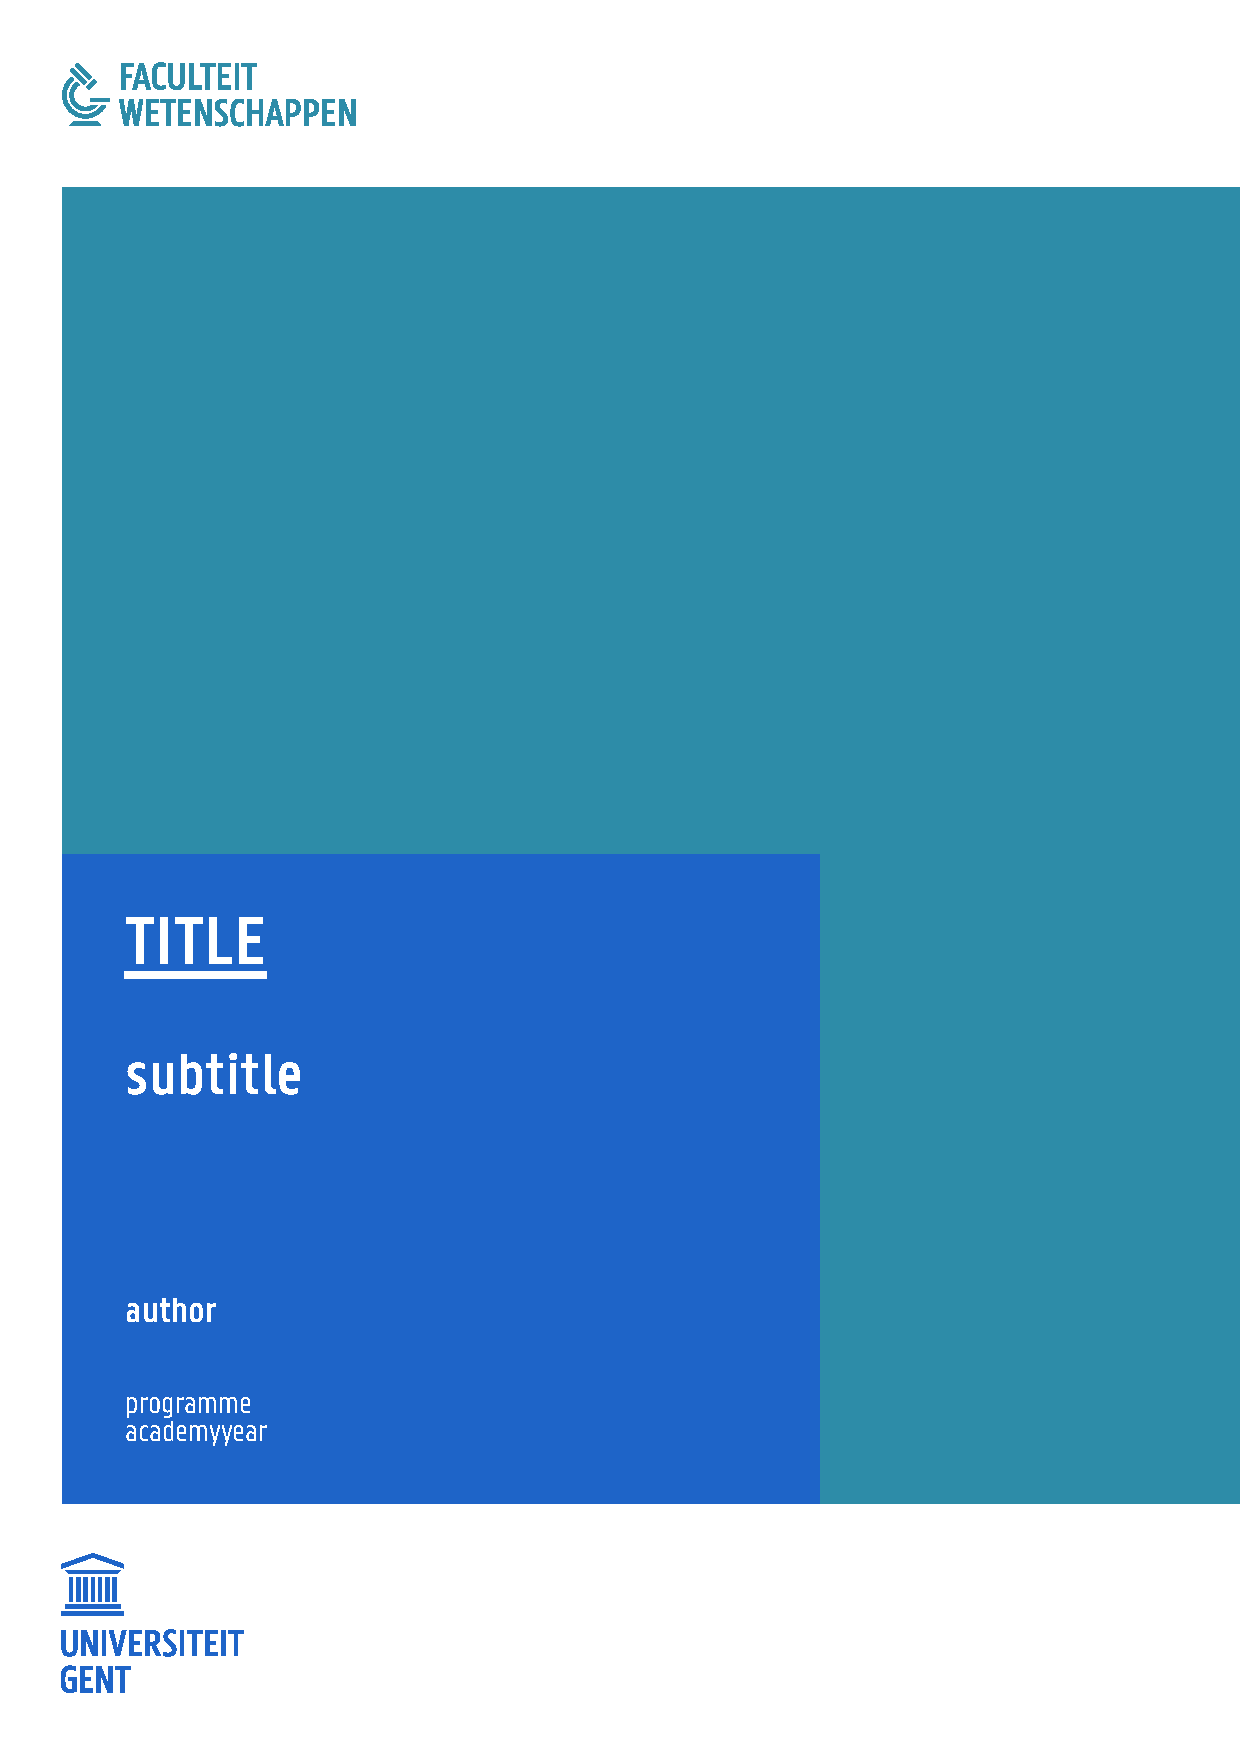
\includegraphics[width=1\textwidth]{ugent2016-title-course.pdf}}
    \end{center}

    \section{Voorblad met stijl \texttt{report}}\label{sec:voorblad-met-stijl-report}
    \begin{center}
        \frame{
\includegraphics[width=1\textwidth]{ugent2016-title-report.pdf}}
    \end{center}

    \section{Voorblad met stijl \texttt{notes}}\label{sec:voorblad-met-stijl-notes}
    \begin{center}
        \frame{
\includegraphics[width=1\textwidth]{ugent2016-title-notes.pdf}}
    \end{center}

    \section{Wijzigingen}\label{sec:wijzigingen}

    Wijzigingen worden bijgehouden op GitHub.

\end{document}
